\documentclass[]{article}
\usepackage[T1]{fontenc}
\usepackage{lmodern}
\usepackage{amssymb,amsmath}
\usepackage{ifxetex,ifluatex}
\usepackage{fixltx2e} % provides \textsubscript
% Set line spacing
% use upquote if available, for straight quotes in verbatim environments
\IfFileExists{upquote.sty}{\usepackage{upquote}}{}
\ifnum 0\ifxetex 1\fi\ifluatex 1\fi=0 % if pdftex
  \usepackage[utf8]{inputenc}
\else % if luatex or xelatex
  \ifxetex
    \usepackage{mathspec}
    \usepackage{xltxtra,xunicode}
  \else
    \usepackage{fontspec}
  \fi
  \defaultfontfeatures{Mapping=tex-text,Scale=MatchLowercase}
  \newcommand{\euro}{€}
\fi
% use microtype if available
\IfFileExists{microtype.sty}{\usepackage{microtype}}{}
\usepackage[margin=1in]{geometry}
\usepackage{color}
\usepackage{fancyvrb}
\newcommand{\VerbBar}{|}
\newcommand{\VERB}{\Verb[commandchars=\\\{\}]}
\DefineVerbatimEnvironment{Highlighting}{Verbatim}{commandchars=\\\{\}}
% Add ',fontsize=\small' for more characters per line
\usepackage{framed}
\definecolor{shadecolor}{RGB}{248,248,248}
\newenvironment{Shaded}{\begin{snugshade}}{\end{snugshade}}
\newcommand{\KeywordTok}[1]{\textcolor[rgb]{0.13,0.29,0.53}{\textbf{{#1}}}}
\newcommand{\DataTypeTok}[1]{\textcolor[rgb]{0.13,0.29,0.53}{{#1}}}
\newcommand{\DecValTok}[1]{\textcolor[rgb]{0.00,0.00,0.81}{{#1}}}
\newcommand{\BaseNTok}[1]{\textcolor[rgb]{0.00,0.00,0.81}{{#1}}}
\newcommand{\FloatTok}[1]{\textcolor[rgb]{0.00,0.00,0.81}{{#1}}}
\newcommand{\CharTok}[1]{\textcolor[rgb]{0.31,0.60,0.02}{{#1}}}
\newcommand{\StringTok}[1]{\textcolor[rgb]{0.31,0.60,0.02}{{#1}}}
\newcommand{\CommentTok}[1]{\textcolor[rgb]{0.56,0.35,0.01}{\textit{{#1}}}}
\newcommand{\OtherTok}[1]{\textcolor[rgb]{0.56,0.35,0.01}{{#1}}}
\newcommand{\AlertTok}[1]{\textcolor[rgb]{0.94,0.16,0.16}{{#1}}}
\newcommand{\FunctionTok}[1]{\textcolor[rgb]{0.00,0.00,0.00}{{#1}}}
\newcommand{\RegionMarkerTok}[1]{{#1}}
\newcommand{\ErrorTok}[1]{\textbf{{#1}}}
\newcommand{\NormalTok}[1]{{#1}}
\usepackage{graphicx}
% Redefine \includegraphics so that, unless explicit options are
% given, the image width will not exceed the width of the page.
% Images get their normal width if they fit onto the page, but
% are scaled down if they would overflow the margins.
\makeatletter
\def\ScaleIfNeeded{%
  \ifdim\Gin@nat@width>\linewidth
    \linewidth
  \else
    \Gin@nat@width
  \fi
}
\makeatother
\let\Oldincludegraphics\includegraphics
{%
 \catcode`\@=11\relax%
 \gdef\includegraphics{\@ifnextchar[{\Oldincludegraphics}{\Oldincludegraphics[width=\ScaleIfNeeded]}}%
}%
\ifxetex
  \usepackage[setpagesize=false, % page size defined by xetex
              unicode=false, % unicode breaks when used with xetex
              xetex]{hyperref}
\else
  \usepackage[unicode=true]{hyperref}
\fi
\hypersetup{breaklinks=true,
            bookmarks=true,
            pdfauthor={barb dornseif - saoirsegirl},
            pdftitle={A Simulation of an Exponential Distribution With an Evaluation Against the Central Limit Theorem (CLT)},
            colorlinks=true,
            citecolor=blue,
            urlcolor=blue,
            linkcolor=magenta,
            pdfborder={0 0 0}}
\urlstyle{same}  % don't use monospace font for urls
\setlength{\parindent}{0pt}
\setlength{\parskip}{6pt plus 2pt minus 1pt}
\setlength{\emergencystretch}{3em}  % prevent overfull lines
\setcounter{secnumdepth}{5}

%%% Change title format to be more compact
\usepackage{titling}
\setlength{\droptitle}{-2em}
  \title{A Simulation of an Exponential Distribution With an Evaluation Against
the Central Limit Theorem (CLT)}
  \pretitle{\vspace{\droptitle}\centering\huge}
  \posttitle{\par}
  \author{barb dornseif - saoirsegirl}
  \preauthor{\centering\large\emph}
  \postauthor{\par}
  \predate{\centering\large\emph}
  \postdate{\par}
  \date{February, 2015}




\begin{document}

\maketitle


\section{Overview}\label{overview}

The Central Limit Theorem states that the distribution of averages
(Means) of Independant and Identically Distributed (IID) variables
becomes that of a Standard Normal as the sample size increases. To test
this theorem, this paper will explore whether a specifically non-Normal
Distribution - the Exponential Distribution - will, when samples are
repeatedly simulated, produce sample Means that will result in a
distribution that is Normal. We will first simulate several samples of
varying sizes and then simulate the average of the Means and Standard
Deviation of repeated samples of 40 random observations of an
Exponential Distribution.

\section{The Simulations}\label{the-simulations}

First we must understand the theoretical nature of the Exponential
Distribution (ED) to understand how it is not Normal. The description of
an Exponential Distribution in wikipedia is as follows:\\``In
probability theory and statistics, the exponential distribution (a.k.a.
negative exponential distribution) is the probability distribution that
describes the time between events in a Poisson process, i.e.~a process
in which events occur continuously and independently at a constant
average rate. It is the continuous analogue of the geometric
distribution, and it has the key property of being memoryless.''

Further we are told that both the Mean and the Standard Deviation are
described as $\frac{1}{\lambda}$. Thus they are equal. For this
excercise we are given a $\lambda = 0.2$. Therefore the theoretical Mean
as well as the Standard Deviation will be 5.

\subsection{Simulation of Theoretical
Distributions}\label{simulation-of-theoretical-distributions}

Pictorially, graphs of the theoretical densities for an Exponential and
Normal distribution where the mean is 5 and the standard deviation = 5
will look like this:

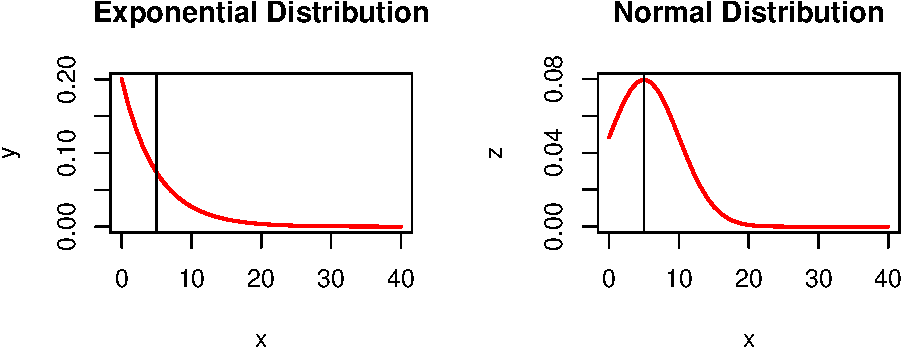
\includegraphics{06_Project1a_files/figure-latex/theoretical_distro-1.pdf}

Figure 1 - Code Chunk 1(CC1)

As we can see in Figure 1, these two density plots are quite different,
so we know that our simulation excercise of averages - when plotted -
will show whether the distribution of sample Means and Standard
Deviations will take on the Exponential or Normal distribution.

Knowing that the size of the sample is implicated in the CLT, first we
will look at three samples of progressively larger sizes, n = c(40, 400,
4000) to see if the sample size itself alters or smoothes the
distribution. We will plot a random sample using our given
$\lambda = 0.2$ and the theoretical Mean and first Standard Deviation
$\mu \pm 5$ to see the center-point and basic spread of the distribution
and overlay our theorectical Exponential Destribution as defined above.

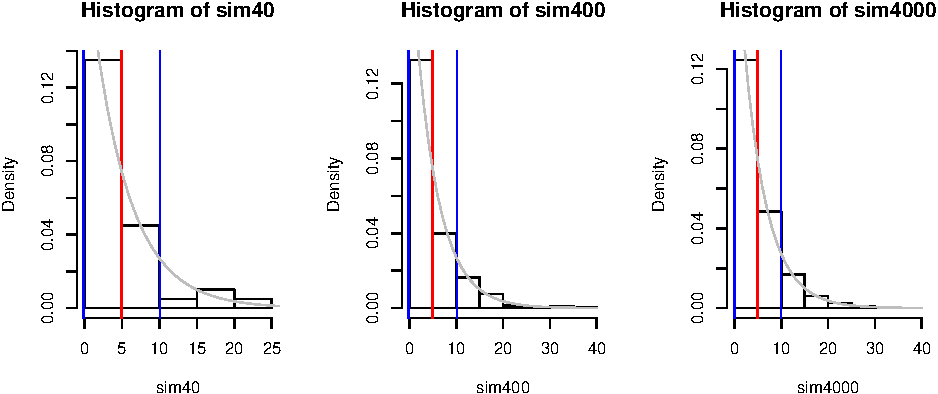
\includegraphics{06_Project1a_files/figure-latex/simulations-1.pdf}

Figure 2 - Code Chunk 2(CC2)

In the figure above, we see that the Mean and Standard Deviation remain
roughly independant of the number of observations in each plot. This
might be better expressed in table form.

\% latex table generated in R 3.1.2 by xtable 1.7-4 package \% Sun Feb
22 00:10:24 2015

\begin{table}[ht]
\centering
\begin{tabular}{rrrr}
  \hline
 & n=40 & n=400 & n=4,000 \\ 
  \hline
Theoretical Means & 5.00 & 5.00 & 5.00 \\ 
  Sample Means & 4.97 & 4.97 & 4.97 \\ 
  Standard Deviation & 5.10 & 5.17 & 4.99 \\ 
   \hline
\end{tabular}
\end{table}

Table 1 - Code Chunk 3(CC3)\\What we observe is that whether the sample
size is 40, 400 or 4,000, the distribution is clear and follows the
theoretical distribution nicely. We also see that the Mean is constant
as we used a seed value to fix the sampling results for replicability.
Thus we should expect that the required n = 40 parameter for the
simulation excercise should produce a reliable test. So let's proceed to
our simulation of the required 1,000 samples and see if the resulting
distribution of the Means from each of our 1,000 samples are Normally
Distributed.

\subsection{Simulation of Mulitple
Samples}\label{simulation-of-mulitple-samples}

As we are given that our samples shall have a $\lambda = 0.2$, and
sample size of 40, our next step is to run 1,000 such samples, calculate
their Means, save those Means into a vector and plot their distribution
to detirmine if they 1) distribute Normally and 2) whether the Mean of
Means and the variance of those Means meets the theoretical expectation
given by the Central Limit Theorem. Mathematically represented as:

\[\frac{\bar X_n - \mu}{\sigma / \sqrt{n}}= \frac{\sqrt n (\bar X_n - \mu)}{\sigma} = \frac{\mbox{Estimate} - \mbox{Mean of estimate}}{\mbox{Std. Err. of estimate}}\]

If we remember that replacing the standard error by its estimated value
doesn't change the CLT a useful way to think about the CLT is that
$\bar X_n$ is approximately $N(\mu, \sigma / \sqrt n)$. So our
expectation is that the Mean will be 5 and the Standard Deviation will
be $5 / \sqrt n$. Given n = 40 we expect 0.79. For simplicity of
plotting we will subtract our Mean from 5 and plot the results against a
Standard Normal Distribution with Mean = 0 to prove the Theorem.

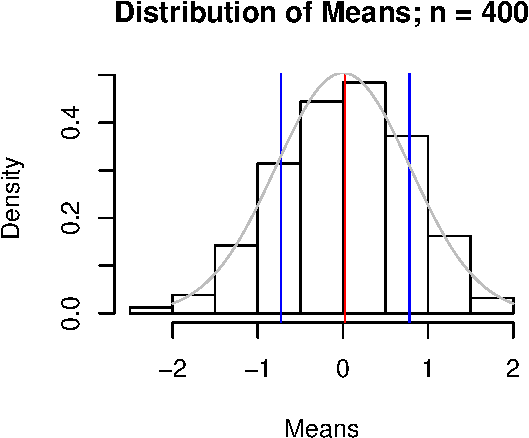
\includegraphics{06_Project1a_files/figure-latex/CLT_Samples-1.pdf}

Figure 3 - Code Chunk 4(CC4)

Our simulation shows that the Mean of Means of 1,000 samples is is
Normally Distributed and imperically the Mean is 0.026 with a Standard
Deviation of 0.755 both of which are very close to our expectation.
Further if we were to increase our number of observations to 400 and
rerun the same code, we would see that the Mean is closer still and the
Standard Deviation even closer to the theoretical expectation as our
last plot shows.

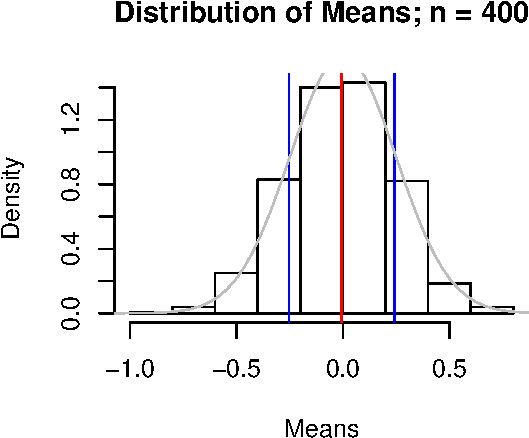
\includegraphics{06_Project1a_files/figure-latex/CLT_Samples400-1.pdf}

Figure 4 - Code Chunk 5(CC5)

Which is in fact what we observe; the Mean is -0.006 with a Standard
Deviation of 0.248. Thus we have proven the CLT works on a distribution
of non-Normal samples to provide a Normal Distribution of Means of those
sample and that as the sample size grows the Normal Distribution will
become more focused on the theoretical Mean of the Population that those
samples are pulled from.

\section{Appendix 1 -- Code chunks for each data simulation, graph and
table}\label{appendix-1-code-chunks-for-each-data-simulation-graph-and-table}

CC1 - Load needed packages, set seed and universal variables. Create
theretical density distributions.

\begin{Shaded}
\begin{Highlighting}[]
\KeywordTok{library}\NormalTok{(ggplot2)}
\KeywordTok{set.seed}\NormalTok{(}\DecValTok{1234}\NormalTok{)}
\NormalTok{lambda <-}\StringTok{ }\FloatTok{0.2}
\NormalTok{n <-}\StringTok{ }\DecValTok{40}
\NormalTok{iter <-}\StringTok{ }\DecValTok{1000}
\NormalTok{x=}\KeywordTok{seq}\NormalTok{(}\DecValTok{0}\NormalTok{,}\DecValTok{40}\NormalTok{)}
\NormalTok{y=}\KeywordTok{dexp}\NormalTok{(x, lambda)}
\KeywordTok{par}\NormalTok{(}\DataTypeTok{mfrow =} \KeywordTok{c}\NormalTok{(}\DecValTok{1}\NormalTok{,}\DecValTok{2}\NormalTok{))}
\KeywordTok{plot}\NormalTok{(x,y,}\DataTypeTok{type=}\StringTok{"l"}\NormalTok{,}\DataTypeTok{lwd=}\DecValTok{2}\NormalTok{,}\DataTypeTok{col=}\StringTok{"red"}\NormalTok{, }\DataTypeTok{main=}\StringTok{"Exponential Distribution"}\NormalTok{)}
\KeywordTok{abline}\NormalTok{(}\DataTypeTok{v=}\DecValTok{5}\NormalTok{)}
\NormalTok{z =}\StringTok{ }\KeywordTok{dnorm}\NormalTok{(x,}\DecValTok{5}\NormalTok{,}\DecValTok{5}\NormalTok{) }\CommentTok{# normal dist mean = 5 and SD = 5}
\KeywordTok{plot}\NormalTok{(x,z,}\DataTypeTok{type=}\StringTok{"l"}\NormalTok{,}\DataTypeTok{lwd=}\DecValTok{2}\NormalTok{,}\DataTypeTok{col=}\StringTok{"red"}\NormalTok{, }\DataTypeTok{main=}\StringTok{"Normal Distribution"}\NormalTok{)}
\KeywordTok{abline}\NormalTok{(}\DataTypeTok{v=}\DecValTok{5}\NormalTok{)}
\end{Highlighting}
\end{Shaded}

CC2 - Simulate samples of random Exponentials with n = c(40,400,4000)

\begin{Shaded}
\begin{Highlighting}[]
\CommentTok{# simulate n random exponentials & calculating the mean and standard deviation of each simulation}
\NormalTok{sim40 <-}\StringTok{ }\KeywordTok{rexp}\NormalTok{(n, lambda); sim400<-}\StringTok{ }\KeywordTok{rexp}\NormalTok{(n*}\DecValTok{10}\NormalTok{, lambda); sim4000<-}\StringTok{ }\KeywordTok{rexp}\NormalTok{(n*}\DecValTok{100}\NormalTok{, lambda)}
\NormalTok{mean40 <-}\StringTok{ }\KeywordTok{mean}\NormalTok{(sim40); mean400 <-}\StringTok{ }\KeywordTok{mean}\NormalTok{(sim40); mean4000 <-}\StringTok{ }\KeywordTok{mean}\NormalTok{(sim40)}
\NormalTok{std40 =}\StringTok{ }\KeywordTok{sqrt}\NormalTok{(}\KeywordTok{var}\NormalTok{(sim40)); std400 =}\StringTok{ }\KeywordTok{sqrt}\NormalTok{(}\KeywordTok{var}\NormalTok{(sim400)); std4000 =}\StringTok{ }\KeywordTok{sqrt}\NormalTok{(}\KeywordTok{var}\NormalTok{(sim4000))}
\CommentTok{# prepare graph layout}
\KeywordTok{par}\NormalTok{(}\DataTypeTok{mfrow =} \KeywordTok{c}\NormalTok{(}\DecValTok{1}\NormalTok{,}\DecValTok{3}\NormalTok{))}
\KeywordTok{hist}\NormalTok{(sim40, }\DataTypeTok{freq=}\OtherTok{FALSE}\NormalTok{); }\KeywordTok{abline}\NormalTok{(}\DataTypeTok{v=}\NormalTok{mean40, }\DataTypeTok{col =} \StringTok{"red"}\NormalTok{)}
\KeywordTok{abline}\NormalTok{(}\DataTypeTok{v=}\NormalTok{mean40-std40, }\DataTypeTok{col=}\StringTok{"blue"}\NormalTok{); }\KeywordTok{abline}\NormalTok{(}\DataTypeTok{v=}\NormalTok{mean40+std40, }\DataTypeTok{col=}\StringTok{"blue"}\NormalTok{)}
\KeywordTok{lines}\NormalTok{(x,y, }\DataTypeTok{col=}\StringTok{"grey"}\NormalTok{)  }
\KeywordTok{hist}\NormalTok{(sim400, }\DataTypeTok{freq=}\OtherTok{FALSE}\NormalTok{); }\KeywordTok{abline}\NormalTok{(}\DataTypeTok{v=}\NormalTok{mean400, }\DataTypeTok{col =} \StringTok{"red"}\NormalTok{)}
\KeywordTok{abline}\NormalTok{(}\DataTypeTok{v=}\NormalTok{mean400-std400, }\DataTypeTok{col=}\StringTok{"blue"}\NormalTok{); }\KeywordTok{abline}\NormalTok{(}\DataTypeTok{v=}\NormalTok{mean400+std400, }\DataTypeTok{col=}\StringTok{"blue"}\NormalTok{)}
\KeywordTok{lines}\NormalTok{(x,y, }\DataTypeTok{col=}\StringTok{"grey"}\NormalTok{) }
\KeywordTok{hist}\NormalTok{(sim4000, }\DataTypeTok{freq=}\OtherTok{FALSE}\NormalTok{); }\KeywordTok{abline}\NormalTok{(}\DataTypeTok{v=}\NormalTok{mean4000, }\DataTypeTok{col =} \StringTok{"red"}\NormalTok{)}
\KeywordTok{abline}\NormalTok{(}\DataTypeTok{v=}\NormalTok{mean4000-std4000, }\DataTypeTok{col=}\StringTok{"blue"}\NormalTok{); }\KeywordTok{abline}\NormalTok{(}\DataTypeTok{v=}\NormalTok{mean4000+std4000, }\DataTypeTok{col=}\StringTok{"blue"}\NormalTok{)}
\KeywordTok{lines}\NormalTok{(x,y, }\DataTypeTok{col=}\StringTok{"grey"}\NormalTok{)}
\end{Highlighting}
\end{Shaded}

CC3 - Present Table of Means and Standard Deviations

\begin{Shaded}
\begin{Highlighting}[]
\KeywordTok{library}\NormalTok{(xtable)}
\NormalTok{Theoretical <-}\StringTok{ }\KeywordTok{c}\NormalTok{(}\DecValTok{5}\NormalTok{, }\DecValTok{5}\NormalTok{, }\DecValTok{5}\NormalTok{)}
\NormalTok{Means <-}\StringTok{ }\KeywordTok{c}\NormalTok{(mean40, mean400, mean4000)}
\NormalTok{SDev <-}\StringTok{ }\KeywordTok{c}\NormalTok{(std40, std400, std4000)}
\NormalTok{table1 <-}\StringTok{ }\KeywordTok{rbind}\NormalTok{(Theoretical, Means, SDev)}
\KeywordTok{rownames}\NormalTok{(table1) <-}\StringTok{ }\KeywordTok{c}\NormalTok{(}\StringTok{"Theoretical Means"}\NormalTok{, }\StringTok{"Sample Means"}\NormalTok{, }\StringTok{"Standard Deviation"}\NormalTok{); }\KeywordTok{colnames}\NormalTok{(table1) <-}\StringTok{ }\KeywordTok{c}\NormalTok{(}\StringTok{"n=40"}\NormalTok{, }\StringTok{"n=400"}\NormalTok{, }\StringTok{"n=4,000"}\NormalTok{)}
\KeywordTok{xtable}\NormalTok{(table1, }\DataTypeTok{format =} \StringTok{"markdown"}\NormalTok{)}
\end{Highlighting}
\end{Shaded}

CC4 - Mean of Means: n=40

\begin{Shaded}
\begin{Highlighting}[]
\KeywordTok{set.seed}\NormalTok{(}\DecValTok{1234}\NormalTok{)}
\NormalTok{Means =}\StringTok{ }\OtherTok{NULL}
\NormalTok{for (i in }\DecValTok{1} \NormalTok{:}\StringTok{ }\NormalTok{iter) \{}
    \NormalTok{Means =}\StringTok{ }\KeywordTok{c}\NormalTok{(Means, }\DecValTok{5} \NormalTok{-}\StringTok{ }\KeywordTok{mean}\NormalTok{(}\KeywordTok{rexp}\NormalTok{(n,lambda)))\}}
\NormalTok{Mean1000 <-}\StringTok{ }\KeywordTok{mean}\NormalTok{(Means)}
\NormalTok{STD1000 <-}\StringTok{ }\KeywordTok{sqrt}\NormalTok{(}\KeywordTok{var}\NormalTok{(Means))}
\KeywordTok{hist}\NormalTok{(Means, }\DataTypeTok{freq =} \OtherTok{FALSE}\NormalTok{, }\DataTypeTok{main =} \StringTok{"Distribution of Means; n = 400"}\NormalTok{)}
\KeywordTok{abline}\NormalTok{(}\DataTypeTok{v =} \NormalTok{Mean1000, }\DataTypeTok{col =} \StringTok{'red'}\NormalTok{)}
\KeywordTok{abline}\NormalTok{(}\DataTypeTok{v =} \NormalTok{Mean1000 -}\StringTok{ }\NormalTok{STD1000, }\DataTypeTok{col =} \StringTok{'blue'}\NormalTok{)}
\KeywordTok{abline}\NormalTok{(}\DataTypeTok{v =} \NormalTok{Mean1000 +}\StringTok{ }\NormalTok{STD1000, }\DataTypeTok{col =} \StringTok{'blue'}\NormalTok{)}
\NormalTok{x=}\KeywordTok{seq}\NormalTok{(-}\DecValTok{2}\NormalTok{,}\DecValTok{2}\NormalTok{, }\DataTypeTok{length=}\DecValTok{100}\NormalTok{) }
\NormalTok{s =}\StringTok{ }\KeywordTok{dnorm}\NormalTok{(x, }\DecValTok{0}\NormalTok{, }\DecValTok{1}\NormalTok{/lambda/}\KeywordTok{sqrt}\NormalTok{(n)) }\CommentTok{# normal dist mean = 5 and Stan error = 5 /sqrt(n)  }
\KeywordTok{lines}\NormalTok{(x,s, }\DataTypeTok{col=}\StringTok{'grey'}\NormalTok{)}
\end{Highlighting}
\end{Shaded}

CC5 - Mean of Means: n=400

\begin{Shaded}
\begin{Highlighting}[]
\KeywordTok{set.seed}\NormalTok{(}\DecValTok{1234}\NormalTok{)}
\NormalTok{n =}\StringTok{ }\DecValTok{400}
\NormalTok{Means =}\StringTok{ }\OtherTok{NULL}
\NormalTok{for (i in }\DecValTok{1} \NormalTok{:}\StringTok{ }\NormalTok{iter) \{}
    \NormalTok{Means =}\StringTok{ }\KeywordTok{c}\NormalTok{(Means, }\DecValTok{5} \NormalTok{-}\StringTok{ }\KeywordTok{mean}\NormalTok{(}\KeywordTok{rexp}\NormalTok{(n,lambda)))\}}
\NormalTok{Mean1000 <-}\StringTok{ }\KeywordTok{mean}\NormalTok{(Means)}
\NormalTok{STD1000 <-}\StringTok{ }\KeywordTok{sqrt}\NormalTok{(}\KeywordTok{var}\NormalTok{(Means))}
\KeywordTok{hist}\NormalTok{(Means, }\DataTypeTok{freq =} \OtherTok{FALSE}\NormalTok{, }\DataTypeTok{main =} \StringTok{"Distribution of Means; n = 400"}\NormalTok{)}
\KeywordTok{abline}\NormalTok{(}\DataTypeTok{v =} \NormalTok{Mean1000, }\DataTypeTok{col =} \StringTok{'red'}\NormalTok{)}
\KeywordTok{abline}\NormalTok{(}\DataTypeTok{v =} \NormalTok{Mean1000 -}\StringTok{ }\NormalTok{STD1000, }\DataTypeTok{col =} \StringTok{'blue'}\NormalTok{)}
\KeywordTok{abline}\NormalTok{(}\DataTypeTok{v =} \NormalTok{Mean1000 +}\StringTok{ }\NormalTok{STD1000, }\DataTypeTok{col =} \StringTok{'blue'}\NormalTok{)}
\NormalTok{x=}\KeywordTok{seq}\NormalTok{(-}\DecValTok{2}\NormalTok{,}\DecValTok{2}\NormalTok{, }\DataTypeTok{length=}\DecValTok{100}\NormalTok{) }
\NormalTok{s =}\StringTok{ }\KeywordTok{dnorm}\NormalTok{(x, }\DecValTok{0}\NormalTok{, }\DecValTok{1}\NormalTok{/lambda/}\KeywordTok{sqrt}\NormalTok{(n)) }\CommentTok{# normal dist mean = 5 and Stan error = 5 /sqrt(n)  }
\KeywordTok{lines}\NormalTok{(x,s, }\DataTypeTok{col=}\StringTok{'grey'}\NormalTok{)}
\end{Highlighting}
\end{Shaded}

\end{document}
